\documentclass[12pt,a4paper]{article}

\usepackage{fontspec}
\setmainfont{arial}
\usepackage{setspace}
\setstretch{1.15}
\usepackage{amsmath}
\usepackage{graphicx}
\usepackage{float}

\title{Fuzzy System}
\author{Arif Suganda\\
        Tadulako University\\
        F5522530002}

\begin{document}
\maketitle
\section{Problem Statement}
Using fuzzy logic, design a fuzzy system to regulate the speed of a fans based on the temperature and humidity of the green house.
The purpose of this system is to maintain the optimal conditions for the plants and reduce the energy consumption of the fans by gradually adjusting the speed of the fan based on the temperature and humidity levels.

\section{Fuzzy Logic Design}
Based on the problem statement, the variables used in this fuzzy system are:
\begin{itemize}
    \item Input variable: Temperature (T) with the range of 0 to 40 degrees Celsius
    \item Input variable: Humidity (H) with the range of 0 to 100 percent
    \item Output variable: Fan Speed (S) with the range of 0 to 100 percent
\end{itemize}

\subsection{Fuzzy Sets and Membership Functions}
For the input variable Temperature (T), we can define the following fuzzy sets:
\begin{itemize}
    \item Low (L): 10 to 22 degrees Celsius
    \item Medium (M): 18 to 28 degrees Celsius
    \item High (H): 24 to 36 degrees Celsius
\end{itemize}
The membership functions for these fuzzy sets can be defined as follows:
\begin{equation}
    \mu_L(T) = \begin{cases}
        1 & \text{if } T \le 10 \\
        \frac{22 - T}{22 - 10} & \text{if } 10 < T < 22 \\
        0 & \text{if } T \ge 22
    \end{cases}
\end{equation}
\begin{equation}
    \mu_M(T) = \begin{cases}
        0 & \text{if } T \le 18 \text{ or } T \ge 28 \\
        \frac{T - 18}{22 - 18} & \text{if } 18 < T < 22 \\
        1 & \text{if } 22 < T < 24 \\
        \frac{28 - T}{28 - 24} & \text{if } 24 \le T < 28 \\
        0 & \text{if } T \ge 28
    \end{cases}
\end{equation}
\begin{equation}
    \mu_H(T) = \begin{cases}
        0 & \text{if } T \le 24 \\
        \frac{T - 24}{36 - 24} & \text{if } 24 < T < 36 \\
        1 & \text{if } T \ge 36
    \end{cases}
\end{equation}

The membership functions can be visualized in the following graph:
\begin{figure}[H]
    \centering
    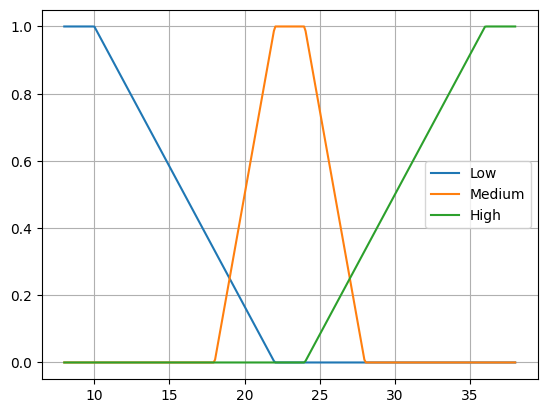
\includegraphics[width=0.8\textwidth]{temperature_membership_functions.png}
    \caption{Membership functions for Temperature (T)}
\end{figure}

For the input variable Humidity (H), we can define the following fuzzy sets:
\begin{itemize}
    \item Low (L): 10 to 30 percent
    \item Medium (M): 20 to 50 percent
    \item High (H): 40 to 60 percent
\end{itemize}
The membership functions for these fuzzy sets can be defined as follows:
\begin{equation}
    \mu_L(H) = \begin{cases}
        1 & \text{if } H \le 30 \\
        \frac{30 - H}{30 - 10} & \text{if } 10 < H < 30 \\
        0 & \text{if } H \ge 30
    \end{cases}
\end{equation}
\begin{equation}
    \mu_M(H) = \begin{cases}
        0 & \text{if } H \le 20 \text{ or } H \ge 50 \\
        \frac{H - 20}{30 - 20} & \text{if } 20 < H < 30 \\
        1 & \text{if } 30 < H < 50 \\
        \frac{50 - H}{50 - 40} & \text{if } 40 \le H < 50 \\
        0 & \text{if } H \ge 50
    \end{cases}
\end{equation}
\begin{equation}
    \mu_H(H) = \begin{cases}
        0 & \text{if } H \le 40 \\
        \frac{H - 40}{60 - 40} & \text{if } 40 < H < 60 \\
        1 & \text{if } H \ge 60
    \end{cases}
\end{equation}

The membership functions can be visualized in the following graph:
\begin{figure}[H]
    \centering
    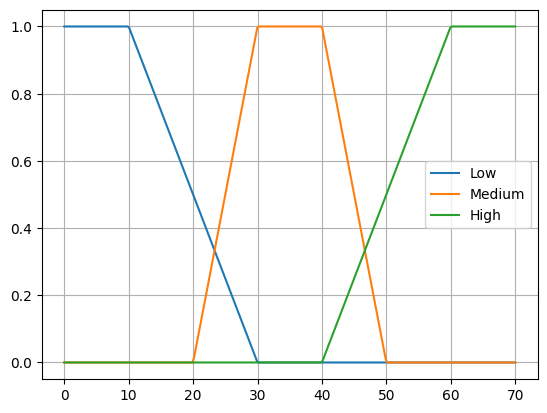
\includegraphics[width=0.8\textwidth]{humidity_membership_functions.png}
    \caption{Membership functions for Humidity (H)}
\end{figure}

For the output variable Fan Speed (S), we can define the following fuzzy sets:
\begin{itemize}
    \item Low (L): 0 to 30 percent
    \item Medium (M): 20 to 70 percent
    \item High (H): 60 to 100 percent
\end{itemize}

\begin{figure}[H]
    \centering
    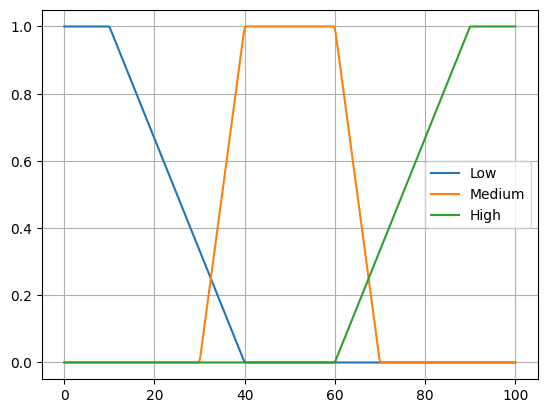
\includegraphics[width=0.8\textwidth]{fan_speed_membership_functions.png}
    \caption{Membership functions for Fan Speed (S)}
\end{figure}

\section{Rule Based}

Rules defined for this fuzzy system are as follows:
\begin{table}[H]
    \centering
    \caption{Fuzzy Logic Rules}
    \begin{tabular}{cccc}
        \hline
        \textbf{Rule} & \textbf{Temperature (T)} & \textbf{Humidity (H)} & \textbf{Fan Speed (S)} \\
        \hline
        1 & Low (L) & Low (L) & Low (L) \\
        2 & Low (L) & Medium (M) & Medium (M) \\
        3 & Low (L) & High (H) & High (H) \\
        4 & Medium (M) & Low (L) & Medium (M) \\
        5 & Medium (M) & Medium (M) & Medium (M) \\
        6 & Medium (M) & High (H) & High (H) \\
        7 & High (H) & Low (L) & High (H) \\
        8 & High (H) & Medium (M) & High (H) \\
        9 & High (H) & High (H) & High (H) \\
        \hline
    \end{tabular}
\end{table}

\section{Manual Calculation}
\subsection{Problem}
For this problem, the temperature is defined as 25 degrees Celsius and the humidity is 38 percent.

\subsection{Fuzzification}
\begin{align}
    \mu\text{T}_L(25) &= 0\\
    \mu\text{T}_M(25) &= \frac{28 - 25}{28 - 24} = \frac{3}{4} = 0.75\\
    \mu\text{T}_H(25) &= \frac{25 - 24}{36 - 24} = \frac{1}{12} \approx 0.08
\end{align}
\begin{align}
    \mu\text{H}_L(38) &= 0\\
    \mu\text{H}_M(38) &= 1\\
    \mu\text{H}_H(38) &= 0\\
\end{align}

\subsection{Rules Evaluation}
Based on the rules defined in the previous section, we can determine the fan speed as follows:
\begin{itemize}
    \item Rule 5: If T is Medium and H is Medium, then S is Medium. The degree of truth for this rule is $\min(\mu\text{T}_M(25), \mu\text{H}_M(38)) = \min(0.75, 1) = 0.75$.
    \item Rule 8: If T is High and H is Medium, then S is High. The degree of truth for this rule is $\min(\mu\text{T}_H(25), \mu\text{H}_M(38)) = \min(0.08, 1) = 0.08$.
\end{itemize}

\subsection{Aggregation}
The aggregated output for the fan speed can be calculated as follows:
\begin{itemize}
    \item Low (L): $\max(0, 0, 0) = 0$
    \item Medium (M): $\max(0, 0.75) = 0.75$
    \item High (H): $\max(0, 0.08) = 0.08$
\end{itemize}

\subsection{Approximate Defuzzification}

Medium:
\begin{align}
    \text{FA}_M(0.75) &= \frac{(70 - 30) + (60 - 40)}{2} \times 0.75 \\
    &= \frac{40 + 20}{2} \times 0.75 \\
    &= 30 \times 0.75 \\
    &= 22.5 \\
    \text{FZ}_M &= \frac{70 + 30}{2} = \frac{100}{2} = 50
\end{align}

High:
\begin{align}
    \text{FA}_H(0.08) &= \frac{(100 - 60) + (100 - 90)}{2} \times 0.08 \\
    &= \frac{40 + 10}{2} \times 0.08 = 25 \times 0.08 \\
    &= 2 \\
    \text{FZ}_H &= \frac{100 + 60}{2} = \frac{160}{2} = 80
\end{align}

Final centroid defuzzification:
\begin{align}
    \text{Centroid} &= \frac{\text{FA}_M(0.75) \times \text{FZ}_M + \text{FA}_H(0.08) \times \text{FZ}_H}{\text{FA}_M(0.75) + \text{FA}_H(0.08)} \\
    &= \frac{22.5 \times 50 + 2 \times 80}{22.5 + 2} \\
    &= \frac{1125 + 160}{24.5} \\
    &\approx \frac{1285}{24.5} \\
    &\approx 52.45
\end{align}

\section{Implementation}

\subsection{Rapidminer}

\subsection{Python}

\begin{verbatim}
import numpy as np
import matplotlib.pyplot as plt

def trapmf(x, a, b, c, d):
    x = np.array(x)
    return np.maximum(
        np.minimum(
            np.minimum((x - a) / (b - a + 1e-9), 1),
            (d - x) / (d - c + 1e-9)
        ),
        0
    )

x_temp = np.linspace(0, 40, 1000)
x_hum = np.linspace(0, 70, 1000)
x_fan = np.linspace(0, 100, 1000)

temp_low = trapmf(x_temp, 0, 0, 10, 22)
temp_med = trapmf(x_temp, 18, 22, 24, 28)
temp_high = trapmf(x_temp, 24, 36, 40, 40)

hum_low = trapmf(x_hum, 0, 0, 10, 30)
hum_med = trapmf(x_hum, 20, 30, 40, 50)
hum_high = trapmf(x_hum, 40, 60, 70, 70)

fan_low = trapmf(x_fan, 0, 0, 10, 40)
fan_med = trapmf(x_fan, 30, 40, 60, 70)
fan_high = trapmf(x_fan, 60, 90, 100, 100)

# Values
temp_val = 25
hum_val = 38

# Fuzzification
def interp_membership(x, mf, val):
    return np.interp(val, x, mf)

t_low = interp_membership(x_temp, temp_low, temp_val)
t_med = interp_membership(x_temp, temp_med, temp_val)
t_high = interp_membership(x_temp, temp_high, temp_val)

h_low = interp_membership(x_hum, hum_low, hum_val)
h_med = interp_membership(x_hum, hum_med, hum_val)
h_high = interp_membership(x_hum, hum_high, hum_val)

# Rule Evaluation (MIN)
rules = []

rules.append((min(t_low, h_low), fan_low))
rules.append((min(t_low, h_med), fan_low))
rules.append((min(t_low, h_high), fan_med))

rules.append((min(t_med, h_low), fan_low))
rules.append((min(t_med, h_med), fan_med))
rules.append((min(t_med, h_high), fan_high))

rules.append((min(t_high, h_low), fan_med))
rules.append((min(t_high, h_med), fan_high))
rules.append((min(t_high, h_high), fan_high))

# Aggregation (MAX)
aggregated = np.zeros_like(x_fan)

for strength, mf in rules:
    clipped = np.minimum(strength, mf)
    aggregated = np.maximum(aggregated, clipped)

# Centroid Defuzzification
def centroid(x, mf):
    return np.sum(x * mf) / np.sum(mf)

result = centroid(x_fan, aggregated)

print(f"Fan Speed = {result:.2f}%")

# Visualization
plt.figure()
plt.plot(x_fan, fan_low, '--', label='Low')
plt.plot(x_fan, fan_med, '--', label='Medium')
plt.plot(x_fan, fan_high, '--', label='High')
plt.plot(x_fan, aggregated, linewidth=2, label='Aggregated')

plt.axvline(result)
plt.title("Fuzzy Output with Centroid")
plt.xlabel("Fan Speed")
plt.ylabel("Membership")
plt.legend()
plt.grid()

plt.show()
\end{verbatim}

Results of this implementation is fan speed \textbf{53.27\%}, the slight difference with the manual calculation is the simplification in the manual calculation.
Compared to it, the Python implementation uses a more accurate method for calculating the aggregated output and the centroid, which can lead to a slightly different result.
The visualization of the fuzzy output with the centroid is shown in the following graph:
\begin{figure}[H]
    \centering
    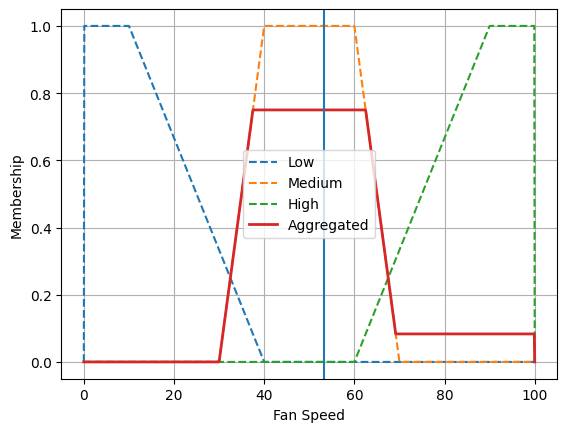
\includegraphics[width=0.8\textwidth]{fuzzy_output.png}
    \caption{Fuzzy Output with Centroid}
\end{figure}

\section{Conclusion}
The result of this implementation shows that the fuzzy system can effectively regulate the fan speed based on the temperature and humidity levels.
The fan speed is calculated to be approximately \textbf{52.45\%} based on the manual calculation and \textbf{53.27\%} based on the Python implementation, which indicates that the system is working as expected.
The slight difference between the manual calculation and the Python implementation can be attributed to the simplifications made in the manual calculation.

\end{document}